\documentclass[a4paper,11pt]{article}
\input{/home/tof/Documents/Cozy/latex-include/preambule_lua.tex}
\newcommand{\showprof}{show them}  % comment this line if you don't want to see todo environment
\fancyhead[L]{Moteurs de recherche}
\newdate{madate}{10}{09}{2020}
%\fancyhead[R]{\displaydate{madate}} %\today
\fancyhead[R]{Seconde - SNT}
%\fancyhead[R]{Première - NSI}
%\fancyhead[R]{Terminale - NSI}
\fancyfoot[L]{~\\Christophe Viroulaud}
\AtEndDocument{\label{lastpage}}
\fancyfoot[C]{\textbf{Page \thepage/\pageref{lastpage}}}
\fancyfoot[R]{\includegraphics[width=2cm,align=t]{/home/tof/Documents/Cozy/latex-include/cc.png}}

\begin{document}
\begin{Form}
\section{Problématique}
Pour naviguer sur internet, il existe principalement deux solutions:
\begin{itemize}
\item en tapant l'\emph{URL (Uniform Ressource Locator)} exacte du site web dans la barre d'adresse du navigateur; exemple: \mbox{\url{https://lyceejaydebeaufort.fr/}},
\item en utilisant un \emph{moteur de recherche} qui trouve les sites en rapport avec un thème donné.
\end{itemize}
\begin{center}
\shadowbox{\parbox{10cm}{\centering Comment fonctionne un moteur de recherche?}}
\end{center}
\section{Différents moteurs}
\begin{aretenir}[]
Un moteur de recherche est un outil qui permet de chercher  des contenus (documents, vidéos, images...) sur le web, à partir de mots clés.
\end{aretenir}
\begin{activite}
\begin{enumerate}
\item Lire l'article suivant \url{https://tinyurl.com/yya3bj9x} et répondre aux questions:
\begin{enumerate}
\item Quel est le moteur le plus utilisé dans le monde?
\item En France, quel pourcentage de parts de marché représente ce moteur (tout appareil confondu)?
\item Citer deux autres moteurs de recherche.
\end{enumerate}
\item Se rendre sur les pages des deux moteurs suivants:
\begin{itemize}
\item \url{https://duckduckgo.com}
\item \url{https://qwant.com}
\end{itemize}
\item Quel principe semble défendre ces deux moteurs de recherche?
\end{enumerate}
\end{activite}
\emph{Qwant} est un moteur de recherche français mis en ligne en 2013. L'extension du moteur de recherche pour le navigateur Mozilla Firefox fait partie de la liste des logiciels libres préconisés par l'État français.\\
Les navigateurs (Firefox, Chrome...) utilisent un moteur de recherche par défaut. Il est possible de modifier ce choix.
\begin{activite}
Depuis les préférences du navigateur:
\begin{enumerate}
\item trouver le moteur de recherche utilisé par défaut,
\item changer de moteur de recherche.
\end{enumerate}
\end{activite}
\section{Indexation}
\subsection{Définition}
\begin{aretenir}[]
Les moteurs analysent, identifient et organisent les documents sur le web pour faciliter une recherche ultérieure.
\end{aretenir}
\begin{activite}
\begin{enumerate}
\item Ouvrir un onglet pour les trois moteurs de recherche suivant:
\begin{itemize}
\item \url{https://duckduckgo.com}
\item \url{https://qwant.com}
\item \url{https://google.com}
\end{itemize}
\item Effectuer la même recherche dans les trois moteurs, par exemple \guill{chaussure de sport}.
\item Les résultats obtenus sont-ils identiques?
\item Pour quelle raison les premiers résultats contiennent le mot \emph{Annonce}?
\end{enumerate}
\end{activite}
\subsection{Algorithme d'indexation}
Le \emph{PageRank} est un algorithme d'analyse des pages web, utilisé par le moteur \emph{Google}. Le principe de base est d'attribuer à chaque page web un score proportionnel au nombre de fois qu'un internaute visite la page quand il clique aléatoirement sur les hyperliens.
\begin{center}
\centering
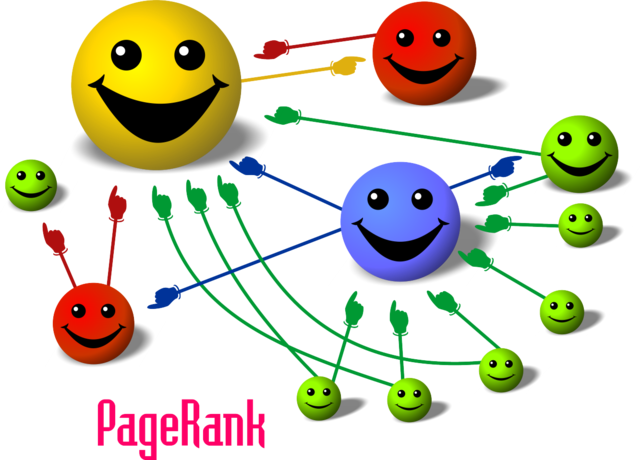
\includegraphics[width=7cm]{ressources/pagerank.png}
\captionof{figure}{Illustration du pagerank}
\label{pagerank}
\end{center}
Plus une page a des hyperliens qui pointent vers elle, plus son score sera élevé et plus elle sera présente dans les premiers résultats de recherche. 
\end{Form}
\end{document}